%%
%% Automatically generated file from Doconce source
%% (https://github.com/hplgit/doconce/)
%%





%-------------------- begin preamble ----------------------

\documentclass[%
twoside,                 % oneside: electronic viewing, twoside: printing
final,                   % or draft (marks overfull hboxes)
chapterprefix=true,      % "Chapter" word at beginning of each chapter
open=right               % start new chapters on odd-numbered pages
10pt]{book}


\listfiles               % print all files needed to compile this document


\usepackage{relsize,epsfig,makeidx,color,setspace,amsmath,amsfonts}
\usepackage[table]{xcolor}
\usepackage{bm,microtype}

\usepackage{anslistings,fancyvrb} % packages needed for verbatim environments


\newenvironment{doconce:movie}{}{}
\newcounter{doconce:movie:counter}




\usepackage[T1]{fontenc}
%\usepackage[latin1]{inputenc}
\usepackage[utf8]{inputenc}
\usepackage{lmodern}         % Latin Modern fonts derived from Computer Modern

% Hyperlinks in PDF:
\definecolor{linkcolor}{rgb}{0,0,0.4}
\usepackage[%
    colorlinks=true,
    linkcolor=linkcolor,
    urlcolor=linkcolor,
    citecolor=black,
    filecolor=black,
    %filecolor=blue,
    pdfmenubar=true,
    pdftoolbar=true,
    bookmarksdepth=3   % Uncomment (and tweak) for PDF bookmarks with more levels than the TOC
            ]{hyperref}
%\hyperbaseurl{}   % hyperlinks are relative to this root

\setcounter{tocdepth}{2}  % number chapter, section, subsection

% Tricks for having figures close to where they are defined:
% 1. define less restrictive rules for where to put figures
\setcounter{topnumber}{2}
\setcounter{bottomnumber}{2}
\setcounter{totalnumber}{4}
\renewcommand{\topfraction}{0.85}
\renewcommand{\bottomfraction}{0.85}
\renewcommand{\textfraction}{0.15}
\renewcommand{\floatpagefraction}{0.7}
% 2. ensure all figures are flushed before next section
\usepackage[section]{placeins}
% 3. enable begin{figure}[H] (often leads to ugly pagebreaks)
%\usepackage{float}\restylefloat{figure}

\usepackage[framemethod=TikZ]{mdframed}

% --- begin definitions of admonition environments ---

% Admonition is an oval gray box
\newmdenv[
  backgroundcolor=gray!5,  %% white with 5%% gray
  skipabove=\topsep,
  skipbelow=\topsep,
  outerlinewidth=0,
  leftmargin=0,
  rightmargin=0,
  roundcorner=5,
  needspace=0pt,
]{graybox1mdframed}

\newenvironment{graybox1admon}[1][]{
\begin{graybox1mdframed}[frametitle=#1]
}
{
\end{graybox1mdframed}
}

% --- end of definitions of admonition environments ---

% prevent orhpans and widows
\clubpenalty = 10000
\widowpenalty = 10000




\newenvironment{doconce:exercise}{}{}
\newcounter{doconce:exercise:counter}

% --- end of standard preamble for documents ---


% insert custom LaTeX commands...

\raggedbottom
\makeindex

%-------------------- end preamble ----------------------

\begin{document}



% ------------------- main content ----------------------


% TITLE: On the Technicalities of Scientific Writing Anno 2012: The Doconce Way
% TITLE: Scientific Writing Anno 2013: The Doconce Way


% ----------------- title -------------------------

\thispagestyle{empty}

\begin{center}
{\LARGE\bf
\begin{spacing}{1.25}
Scientific Writing and Publishing Anno 2013
\end{spacing}
}
\end{center}

% ----------------- author(s) -------------------------

\begin{center}
{\bf Hans Petter Langtangen${}^{}$} \\ [0mm]
\end{center}

\begin{center}
% List of all institutions:
\end{center}
% ----------------- end author(s) -------------------------


\begin{center}
Jan 8, 2014
\end{center}

\vspace{1cm}



\begin{center}  % inline figure
  \centerline{
\includegraphics[width=0.5\linewidth]{fig/doconce1b.png}}
\end{center}



% !split
\section*{Scientific writing = {\LaTeX}}

\begin{itemize}
 \item Pre 1980: Handwriting + publisher (paper or book)

 \item Post 1984: scientists write TeX and {\LaTeX}

 \item Post 1995: publish {\LaTeX} on the web or in journals and books
\end{itemize}

\noindent
\begin{latexcode:nt}
\providecommand{\shadedskip}{}
\definecolor{shadecolor}{rgb}{0.87843, 0.95686, 1.0}
\renewenvironment{shadedskip}{
\def\FrameCommand{\colorbox{shadecolor}}\FrameRule0.6pt
\MakeFramed {\FrameRestore}\vskip3mm}{\vskip0mm\endMakeFramed}
\providecommand{\shadedquoteBlue}{}
\renewenvironment{shadedquoteBlue}[1][]{
\bgroup\rmfamily\fboxsep=0mm\relax
\begin{shadedskip}
\list{}{\parsep=-2mm\parskip=0mm\topsep=0pt\leftmargin=2mm
\rightmargin=2\leftmargin\leftmargin=4pt\relax}
\relax}{\endlist\end{shadedskip}\egroup}\begin{shadedquoteBlue}
\fontsize{9pt}{9pt}
\begin{Verbatim}
print 'Hello, World!'
\end{Verbatim}
\end{latexcode:nt}

Big late 1990s question: Will MS Word replace {\LaTeX}? It never did!

% !split
\section*{Scientific publishing needs to address new media}

% !bslidecell 00 0.4

\begin{center}  % inline figure
  \centerline{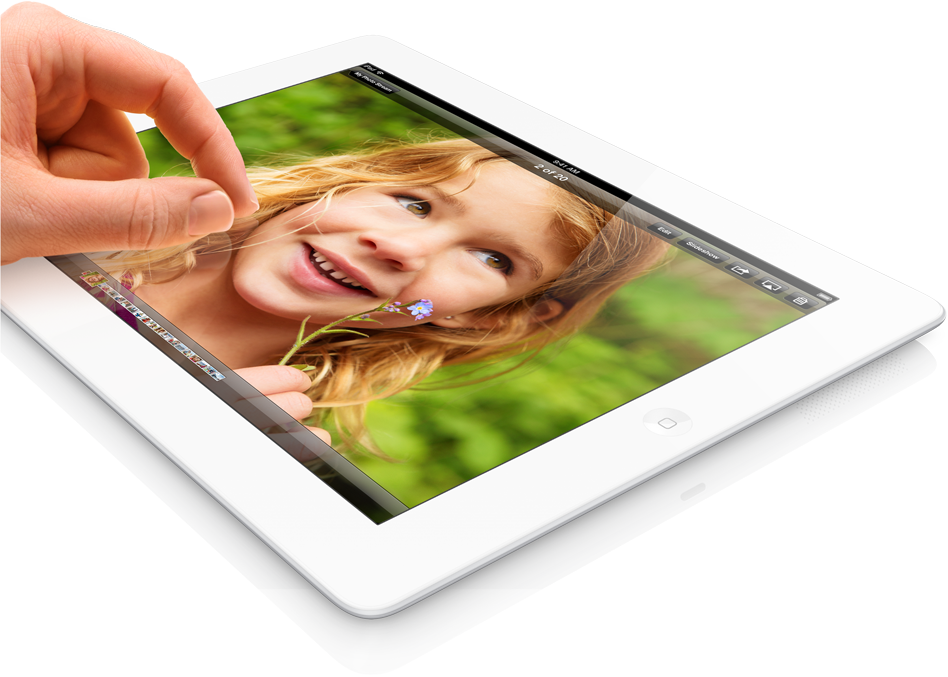
\includegraphics[width=0.8\linewidth]{fig/ipad.png}}
\end{center}



\begin{center}  % inline figure
  \centerline{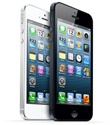
\includegraphics[width=0.3\linewidth]{fig/iphones.jpg}}
\end{center}


% FIGURE: [fig/mbair, width=400]

% !eslidecell

% !bslidecell 01 0.6

\begin{center}  % inline figure
  \centerline{
\includegraphics[width=0.7\linewidth]{fig/imac.png}}
\end{center}

% !eslidecell

% !split
\section*{The book will probably survive}


\begin{center}  % inline figure
  \centerline{
\includegraphics[width=0.9\linewidth]{fig/oldbooks.jpg}}
\end{center}


% !split
\section*{The classical report will survive}

% !bslidecell 00

\begin{center}  % inline figure
  \centerline{
\includegraphics[width=1.2\linewidth]{fig/latex_thesis.jpg}}
\end{center}

% !eslidecell

% !bslidecell 01

\begin{center}  % inline figure
  \centerline{
\includegraphics[width=1.2\linewidth]{fig/latex_paper1.png}}
\end{center}

% !eslidecell

% !split
% * Scientific writing = lecture notes, slides, reports, thesis, books,  ...
% * (Journal papers typeset by journals are out of scope)

\section*{Scope of this presentation}

\begin{itemize}
  \item Focus: documents with \textcolor{red}{much} \emph{math} and \emph{computer code}

  \item Key question: What tools should I use for scientific writing?
\end{itemize}

\noindent

\begin{graybox1admon}[]
The default answer is {\LaTeX}, but there are many
recent popular alternative tools: HTML w/MathJax,
Sphinx, Markdown, MediaWiki, IPython notebook.
\end{graybox1admon}




% !bslidecell 00 0.25

\begin{center}  % inline figure
  \centerline{
\includegraphics[width=0.3\linewidth]{fig/LaTeX_logo.jpg}}
\end{center}

% !eslidecell

% !bslidecell 01 0.25

\begin{center}  % inline figure
  \centerline{
\includegraphics[width=0.2\linewidth]{fig/MS_Word_logo.jpg}}
\end{center}

% !eslidecell

% !bslidecell 02 0.5

\begin{center}  % inline figure
  \centerline{
\includegraphics[width=0.4\linewidth]{fig/sphinx_logo.png}}
\end{center}

% !eslidecell

% !bslidecell 10 0.25

\begin{center}  % inline figure
  \centerline{
\includegraphics[width=0.2\linewidth]{fig/markdown_logo.jpg}}
\end{center}

% !eslidecell

% !bslidecell 11 0.25

\begin{center}  % inline figure
  \centerline{
\includegraphics[width=0.2\linewidth]{fig/MediaWiki_logo.jpg}}
\end{center}

% !eslidecell

% !bslidecell 12 0.5

\begin{center}  % inline figure
  \centerline{
\includegraphics[width=0.6\linewidth]{fig/IPython_logo.png}}
\end{center}

% !eslidecell

% !split
\section*{Does your scientific writing today need to address new media (in the future)?}

% Insert links here to reports

% !bslidecell 00 0.4
\begin{itemize}
 \item BW paper

 \item Color paper

 \item Slides

 \item Web w/design

 \item Wiki

 \item Blog

 \item Notebook

 \item ...
\end{itemize}

\noindent
% !eslidecell

% !bslidecell 01 0.6

\begin{center}  % inline figure
  \centerline{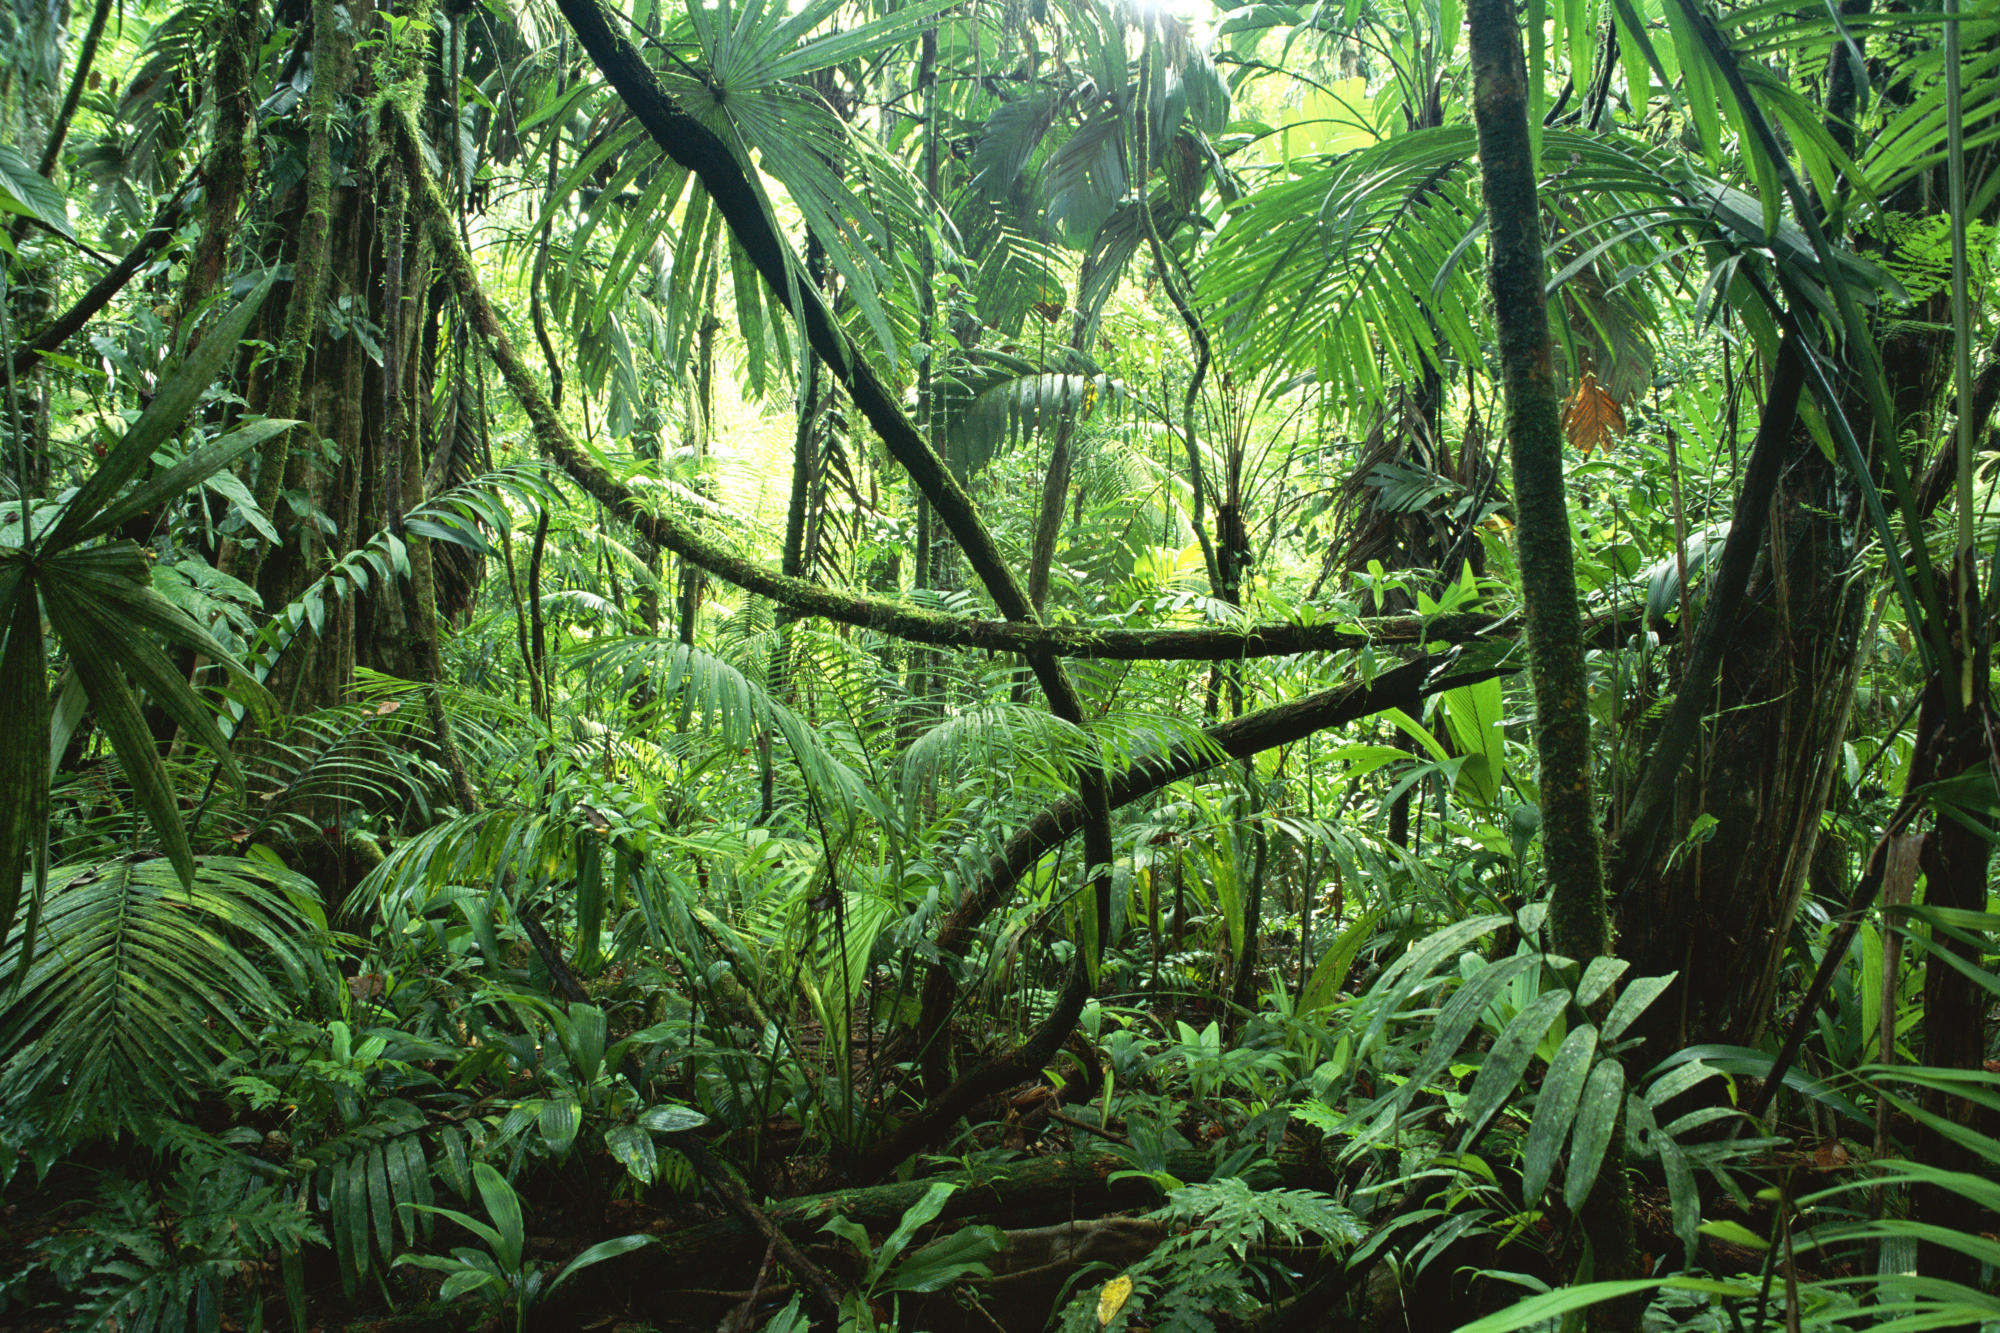
\includegraphics[width=0.9\linewidth]{fig/jungle_with_mess.jpg}}
\end{center}

% !eslidecell

% !split

\section*{Can we factor pieces from a heterogeneous world to one coherent piece in the future?}

When I write some scientific material,

\begin{itemize}
 \item a {\LaTeX} document,

 \item a blog post (HTML),

 \item some web pages (HTML),

 \item a Sphinx document,

 \item an IPython notebook,

 \item some Markdown files,
\end{itemize}

\noindent
and later want to collect the pieces into a larger document, maybe
some book, or one big web document, or a set of slides,
is that at all feasible?

% !bpop highlight-red
Probably not, but I have a solution :-)
% !epop

% !split
\section*{Popular tools anno 2013 and their math support}

% !bpop
\begin{itemize}
 \item \textbf{LaTeX}: de facto standard for math-instensive documents

 \item \textbf{pdfLaTeX}, \textbf{XeLaTeX}, \textbf{LuaLaTeX}: takes over (figures in png, pdf) - use these!

 \item \textbf{MS Word}: too clicky math support and ugly fonts, but much used

 \item \textbf{HTML with MathJax}: "full" {\LaTeX} \emph{math}, but much tagging

 \item \textbf{Sphinx}:
   somewhat limited {\LaTeX} math support, but great support for web design,
   and less tagged than HTML

 \item \textbf{reStructuredText}: similar to Sphinx, but no math support, transforms to
   lots of formats ({\LaTeX}, HTML, XML, Word, OpenOffice, ...)

 \item \textbf{Markdown}: somewhat limited {\LaTeX} math support, but minor tagging,
   transforms to lots of formats ({\LaTeX}, HTML, XML, Word, OpenOffice, ...)

 \item \textbf{IPython notebooks}: Markdown code/math,
   combines Python code, interactivity, and
   visualization, but requires all code snippets to sync together

 \item \textbf{MediaWiki}: quite good {\LaTeX} math support (cf.~Wikipedia/Wikibooks)

 \item Other \textbf{wiki} formats: no math support, great for collaborative editing

 \item \textbf{Wordpress}: supports {\LaTeX} \emph{formulas} only, but good blog post support

 \item \textbf{Google blogger}: supports full HTML with MathJax

 \item \textbf{Epydoc}: old tool for Python code documentation

 \item \textbf{Plain text for email}: no math, just raw {\LaTeX}, and no tagging
\end{itemize}

\noindent
% !epop

% !split

\section*{{\LaTeX} is very rich; other tools support much less}

\begin{itemize}
 \item {\LaTeX} inline math: works with all ({\LaTeX}, MathJax, Sphinx, Markdown, MediaWiki)

 \item {\LaTeX} equation math:
\begin{itemize}

    \item \textbf{LaTeX}: \Verb!equation*!, \Verb!equation!, \Verb!align*!, \Verb!align! +
      \Verb!eqnarray!, \Verb!split!, \Verb!alignat!, ... (numerous!)

    \item \textbf{MathJax}: \Verb!equation*!, \Verb!equation!, \Verb!align*!, \Verb!align!

    \item \textbf{MediaWiki}: \Verb!equation*!, \Verb!equation!, \Verb!align*!, \Verb!align!

    \item \textbf{Sphinx}: \Verb!equation*!, \Verb!equation!, \Verb!align*!

    \item \textbf{Markdown}: \Verb!equation*!, \Verb!equation!, \Verb!eqnarray*!, \Verb!align*! (but no labels)
\end{itemize}

\noindent
\end{itemize}

\noindent
% !split
\section*{{\LaTeX} is very rich; other tools support much less}

% !bpop
\begin{itemize}
 \item Figures: all

 \item Subfigures: {\LaTeX} (\Verb!subfigure!)

 \item Movies: {\LaTeX}, raw HTML

 \item Floating computer code: {\LaTeX}; fixed computer code: all

 \item Interactive programs: Sphinx, IPython notebook, raw HTML

 \item Floating tables: {\LaTeX}; fixed tables: all

 \item Algorithms: {\LaTeX}

 \item Margin notes: {\LaTeX}, HTML with tailored css code

 \item Page references: {\LaTeX}

 \item Footnotes: {\LaTeX}, Sphinx, reStructuredText, MediaWiki

 \item Bibliography: {\LaTeX}, Sphinx, reStructuredText, MediaWiki

 \item Hyperlinks: all (but not on paper!)
\end{itemize}

\noindent
% !epop

% !bpop
Conclusion: Highly non-trivial to translate a {\LaTeX} document into something
based on HTML and vice versa.
% !epop

% !split
\section*{Typesetting concerns I}

% !bpop
\begin{itemize}
 \item Sphinx refers to figures by the caption (has to be short!) and
   strips away any math notation (avoid that!).

 \item Sphinx refers to sections by the title, but removes math in the
   reference, so avoid math in headlines.

 \item Tables cannot be referred to by numbers and have to appear at
   fixed positions in the text.

 \item Computer code has to appear at fixed positions in the text.

 \item Algorithms must be written up using basic elements like lists or
   paragraphs with headings.

 \item Recipes are often typeset as enumerated lists. For recipes with
   code or math blocks: drop the list (gives problems in some formats)
   and use paragraph (or subsubsection) headings with "Step 1.",
   "Step 2.", etc.
\end{itemize}

\noindent
% !epop

% !split
\section*{Typesetting concerns II}

% !bpop
\begin{itemize}
 \item Footnotes must appear as part of the running text (e.g., sentences
   surrounded by parenthesis), since only a few formats support footnotes.

 \item Sphinx does not handle code blocks where the first line is indented.

 \item Multiple plots in the same figure: mount the plots to one image
   file and include this (\Verb!montage! for png, gif, jpeg; \Verb!pdftk!, \Verb!pdfnup!,
   and \Verb!pdfcrop! for PDF).

 \item If you need several equations \emph{numbered} in an \Verb!align! environment,
   recall that Sphinx, Markdown, and MediaWiki cannot handle this,
   although they have {\LaTeX} math support.

 \item Markdown tolerates labels in equations but cannot refer to them.
\end{itemize}

\noindent
% !epop

% Not valid anymore:
% Keys for items in the bibliography are made visible by Sphinx so
% "bibitems" a la \textsc{Bib}\negthinspace{\TeX} must look sensible and consistent.

% !split
\section*{Typesetting concerns III}

% !bpop
\begin{itemize}
 \item Index words can appear anywhere in {\LaTeX}, but should be outside
   paragraphs in other tools.

 \item References to tables, program code and algorithms can only be
   made in {\LaTeX}.

 \item Figures are floating in {\LaTeX}, but fixed in other tools, so place
   figures exactly where they are needed the first time.

 \item Curve plots with color lines do not work well in black-and-white
   printing. Make sure plots makes sense in color and BW (e.g., by
   using colors \emph{and} markers).
\end{itemize}

\noindent
% !epop

% !split
\section*{Solution I: Use a format that translates to many}

\begin{itemize}
 \item Sphinx can do nice HTML, {\LaTeX}, epub, (almost) plain text,
   man pages, Gnome devhelp files, Qt help files, texinfo, JSON

 \item Markdown can do {\LaTeX}, HTML, MS Word, OpenOffice, XML,
   reStructuredText, epub, DocBook, ... but not Sphinx

 \item IPython notebook: can do {\LaTeX}, reStructuredText, HTML, PDF,
   Python script

 \item Sphinx and Markdown has some limited math support
\end{itemize}

\noindent
% !split
\section*{Solution II: Use Doconce}

\href{{http://hplgit.github.io/doconce/doc/web/index.html}}{Doconce}
offers minimalistic typing, great flexibility wrt format,
especially for scientific writing with \emph{much math and code}.

\begin{itemize}
 \item Can generate {\LaTeX}, HTML, Sphinx, Markdown, MediaWiki, Google wiki,
   Creole wiki, reST, plain text

 \item Made for large science books \emph{and} small notes

 \item Targets paper and screen

 \item Many special features (code snippets from files, embedded movies,
   admonitions, modern {\LaTeX} layouts, ...)

 \item Very effective for generating slides from ordinary text

 \item Applies Mako: Doconce text is a program (!)

 \item Much like Markdown, less tagged than {\LaTeX}, HTML, Sphinx
\end{itemize}

\noindent
% !split
\section*{Doconce demos}

\href{{http://hplgit.github.com/teamods/writing_reports/}}{\nolinkurl{http://hplgit.github.com/teamods/writing_reports/}}

\begin{itemize}
 \item LaTeX-based PDF \href{{http://hplgit.github.com/teamods/writing_reports/_static/report.pdf}}{for screen}, \href{{http://hplgit.github.com/teamods/writing_reports/_static/report_4printing.pdf}}{for printing}, \href{{http://hplgit.github.com/teamods/writing_reports/_static/report_4phone.pdf}}{for phone}

 \item \href{{http://hplgit.github.com/teamods/writing_reports/_static/report_do.html}}{Plain HTML} or with a \href{{http://hplgit.github.com/teamods/writing_reports/_static/report_vagrant.html}}{template} or \href{{http://hplgit.github.com/teamods/writing_reports/_static/report_github_minimal.html}}{another template} or \href{{http://hplgit.github.com/teamods/writing_reports/_static/report_solarized.html}}{solarized}

 \item Sphinx: \href{{http://hplgit.github.com/teamods/writing_reports/_static/sphinx-agni/index.html}}{agni}, \href{{http://hplgit.github.com/teamods/writing_reports/_static/sphinx-pyramid/report.html}}{pyramid}, \href{{http://hplgit.github.com/teamods/writing_reports/_static/sphinx-classy/report.html}}{classy}, \href{{http://hplgit.github.com/teamods/writing_reports/_static/sphinx-fenics_minimal/report.html}}{fenics}, \href{{http://hplgit.github.com/teamods/writing_reports/_static/sphinx-redcloud/report.html}}{redcloud}

 \item HTML for \href{{http://doconce-report-demo.blogspot.no/}}{Google} or \href{{http://doconcereportdemo.wordpress.com/}}{Wordpress} for blog posts

 \item \href{{http://doconcedemo.shoutwiki.com/wiki/Doconce_demo_page}}{MediaWiki} (Wikipedia, Wikibooks, etc)

 \item Doconce \href{{http://hplgit.github.com/teamods/writing_reports/_static/report.do.txt.html}}{source code} and \href{{http://hplgit.github.io/doconce/doc/pub/tutorial/html/index.html}}{tutorial}
\end{itemize}

\noindent
% !split
\section*{Doconce disclaimer}

\begin{itemize}
 \item Based on text transformations (reg.exp.) so valid syntax may
   occasionally give problems
% * Actively developed and maintained, but one-man show
\end{itemize}

\noindent

\begin{graybox1admon}[Doconce divorce.]
At any time one can divorce from Doconce and marry one of the output
formats, such as {\LaTeX} or Sphinx. The generated code is clean.
\end{graybox1admon}



% !split
\section*{Doconce experience: code generation is a great thing}


\begin{graybox1admon}[]

Regardless of what format you write in, introduce a step where
you can generate (parts of) the syntax.

\begin{itemize}
 \item Use a preprocessor a la Mako

 \item Write your own read-and-generate code

 \item or both (like Doconce)
\end{itemize}

\noindent
Advantages:

\begin{itemize}
 \item Less writing

 \item Repository of syntax for nice constructions

 \item Implements structure/rules across documents

 \item Easier to change layout/structure
\end{itemize}

\noindent
\end{graybox1admon}



% !split
\subsection*{Example: generate reveal.js or deck.js slides from HTML}

\begin{itemize}
 \item Write the content of each slide in plain HTML(5)

 \item Use e.g. \Verb!#slide! as delimiter between slides

 \item Read file, splitting wrt \Verb!#slide! yields a list of
   slides (HTML code)

 \item For a specific format (reveal.js, deck.js, csss, ...):
\begin{itemize}

    \item write header

    \item for slide in slides:
\begin{itemize}

      \item embed slide in correct HTML code

\end{itemize}

\noindent
    \item write footer
\end{itemize}

\noindent
\end{itemize}

\noindent
\begin{Verbatim}[numbers=none,fontsize=\fontsize{9pt}{9pt},baselinestretch=0.95]
<h2>Scope of this presentation</h2>
<ul>
  <li>Focus: documents with much <em>math</em> and
      <em>computer code</em>
  <li>Key question: What tools should I use for scientific writing?
</ul>
<p><div class="alert">
The default answer is LaTeX.
</div>
\end{Verbatim}

% !split

% latex interprets 9 = as chapter and then needs book style...
\section*{A tour of Doconce}

% !split
\section*{Title, authors, date, toc}

\begin{Verbatim}[numbers=none,fontsize=\fontsize{9pt}{9pt},baselinestretch=0.95]
TITLE: Some Title
AUTHOR: name1 at institution1, with more info & institution2
AUTHOR: name2 email:name2@web.com at institution
DATE: today

# A table of contents is optional:
TOC: on
\end{Verbatim}


\begin{graybox1admon}[Notice.]
Title and authors must have all information \emph{on a single line}!
\end{graybox1admon}



% !split
\section*{Abstract}

\begin{Verbatim}[numbers=none,fontsize=\fontsize{9pt}{9pt},baselinestretch=0.95]
__Abstract.__
Here goes the abstract...
\end{Verbatim}

Or:
\begin{Verbatim}[numbers=none,fontsize=\fontsize{9pt}{9pt},baselinestretch=0.95]
__Summary.__
Here goes the summary...
\end{Verbatim}


% !split
\section*{Section headings}

Headings are surrounded by \Verb!=! signs:
\begin{Verbatim}[numbers=none,fontsize=\fontsize{9pt}{9pt},baselinestretch=0.95]
========= This is an H1/chapter heading =========

======= This is an H2/section heading =======

===== This is an H3/subsection heading =====

=== This is an H4/paragraph heading ===

__This is a paragraph heading.__
\end{Verbatim}

Result:

\chapter{This is an H1/chapter heading}

\section*{This is an H2/section heading}

\subsection*{This is an H3/subsection heading}

\paragraph{This is an H4/paragraph heading.}
\paragraph{This is a paragraph heading.}
% !split
\section*{Markup and lists}

\begin{Verbatim}[numbers=none,fontsize=\fontsize{9pt}{9pt},baselinestretch=0.95]
 * Bullet list items start with `*`
   and may span several lines
 * *Emphasized words* are possible
 * _Boldface words_ are also possible
 * color{red}{colored words} too
 * `inline verbatim code` is featured
   o and sublists with enumerated items starting with `o`
   o items are just indented as you would do in email
\end{Verbatim}

This gets rendered as

\begin{itemize}
 \item Bullet lists start with \Verb!*!
   and may span several lines

 \item \emph{Emphasized words} are possible

 \item \textbf{Boldface words} are also possible

 \item \textcolor{red}{colored words} too

 \item \Verb!inline verbatim code! is featured
\begin{enumerate}

  \item and sublists with enumerated items starting with \Verb!o!

  \item items are just indented as you would do in email
\end{enumerate}

\noindent
\end{itemize}

\noindent
% !split
\section*{Labels, references, index items}

\begin{Verbatim}[numbers=none,fontsize=\fontsize{9pt}{9pt},baselinestretch=0.95]
# Insert index items in the source
idx{key word1} idx{key word2}

# Label
===== Some section =====
label{this:section}

# Make reference
As we saw in Section ref{this:section}, references, index
items and labels follow a syntax similar to LaTeX
but without backslashes.

# Make reference to equations
See (ref{eq1})-(ref{myeq}).

# Make hyperlink
"some link text": "https://github.com/hplgit/doconce"

# Hyperlink with complete URL as link text
URL: "https://github.com/hplgit/doconce"
\end{Verbatim}

% !split
\section*{Figures and movies}


\begin{graybox1admon}[Important:]
Figures with HTML and {\LaTeX} size info, and caption: \emph{everything on one line}
\end{graybox1admon}



\begin{Verbatim}[numbers=none,fontsize=\fontsize{9pt}{9pt},baselinestretch=0.95]
FIGURE: [figdir/myfig, width=300 frac=1.2] My caption. label{fig1}
\end{Verbatim}

Movies are also supported:

\begin{Verbatim}[numbers=none,fontsize=\fontsize{9pt}{9pt},baselinestretch=0.95]
MOVIE: [http://youtu.be/IDeGDFZSYo8, width=420 height=315]
\end{Verbatim}
and rendered as


\begin{doconce:movie}
\refstepcounter{doconce:movie:counter}
\begin{center}
\href{{http://youtube.com/IDeGDFZSYo8}}{\nolinkurl{http://youtube.com/IDeGDFZSYo8}}
\end{center}
\end{doconce:movie}


% !split
\section*{Math}

Inline math as in {\LaTeX}:

\begin{Verbatim}[numbers=none,fontsize=\fontsize{9pt}{9pt},baselinestretch=0.95]
...where $a=\int_{\Omega}fdx$ is an integral.
\end{Verbatim}
gets rendered as ...where $a=\int_{\Omega}fdx$ is an integral.


An equation environment is surrounded by \Verb~!bt~ and \Verb~!et~ tags,
the rest is plain {\LaTeX}:

\begin{Verbatim}[numbers=none,fontsize=\fontsize{9pt}{9pt},baselinestretch=0.95]
!bt
\begin{align}
\frac{\partial u}{\partial t} &= \nabla^2 u,
label{a:eq}\\ 
\nabla\cdot\pmb{v} & = 0
label{b:eq}
\end{align}
!et
\end{Verbatim}
which is rendered as

\begin{align}
\frac{\partial u}{\partial t} &= \nabla^2 u,
\label{a:eq}\\ 
\nabla\cdot\pmb{v} & = 0
\label{b:eq}
\end{align}

% !split
\section*{Math flexibility}

Limit math environments to

\begin{Verbatim}[numbers=none,fontsize=\fontsize{9pt}{9pt},baselinestretch=0.95]
\[ ... \]

\begin{equation*}
\end{equation*}

\begin{equation}
\end{equation}

\begin{align*}
\end{align*}

\begin{align}
\end{align}
\end{Verbatim}


\begin{graybox1admon}[Doconce fix of shortcomings.]
\begin{itemize}
 \item Sphinx, Markdown, and MediaWiki cannot have
   \Verb!align! with labels

 \item MathJax (HTML, Sphinx, Markdown, Mediawiki, ...) cannot
   handle equation references across web pages
\end{itemize}

\noindent
\end{graybox1admon}



% !split
\section*{Displaying code}

Code is enclosed in \Verb~!bc~ and \Verb~!ec~ tags:

\begin{Verbatim}[numbers=none,fontsize=\fontsize{9pt}{9pt},baselinestretch=0.95]
!bc pycod
def solver(I, a, T, dt, theta):
    """Solve u'=-a*u, u(0)=I, for t in (0,T] with steps of dt."""
    dt = float(dt); N = int(round(T/dt)); T = N*dt
    u = zeros(N+1); t = linspace(0, T, N+1)

    u[0] = I
    for n in range(0, N):
        u[n+1] = (1 - (1-theta)*a*dt)/(1 + theta*dt*a)*u[n]
    return u, t
!ec
\end{Verbatim}
This gets rendered as

\begin{python:nt}
def solver(I, a, T, dt, theta):
    """Solve u'=-a*u, u(0)=I, for t in (0,T] with steps of dt."""
    dt = float(dt); N = int(round(T/dt)); T = N*dt
    u = zeros(N+1); t = linspace(0, T, N+1)

    u[0] = I
    for n in range(0, N):
        u[n+1] = (1 - (1-theta)*a*dt)/(1 + theta*dt*a)*u[n]
    return u, t
\end{python:nt}



% !split
\section*{Copying code from source files}

We recommend to copy as much code as possible directly from the
source files:

\begin{Verbatim}[numbers=none,fontsize=\fontsize{9pt}{9pt},baselinestretch=0.95]
@@@CODE path/to/file
@@@CODE path/to/file   fromto: start-regex@end-regex
\end{Verbatim}
For example, copying a code snippet starting with \Verb!def solver(! and
ending with (line not included) \Verb!def next(x, y,! is specified by
start and end regular expressions:

\begin{Verbatim}[numbers=none,fontsize=\fontsize{9pt}{9pt},baselinestretch=0.95]
@@@CODE src/dc_mod.py  fromto: def solver\(@def next\(x,\s*y,
\end{Verbatim}

% !split
\section*{Typesetting of code is implied by the file extension}

\begin{itemize}
 \item \Verb!.py!: \Verb!pypro! if complete file, \Verb!pycod! if snippet

 \item \Verb!.pyopt!: visualized execution via the \href{{http://pythontutor.com}}{Online Python Tutor}

 \item \Verb!.f!, \Verb!.f90!, \Verb!f.95!: \Verb!fpro! and \Verb!fcod!

 \item \Verb!.cpp!, \Verb!.cxx!: \Verb!cpppro! and \Verb!cppcod!

 \item \Verb!.c!: \Verb!cpro! and \Verb!ccod!

 \item \Verb!.*sh!: \Verb!shpro! and \Verb!shcod!

 \item \Verb!.m!: \Verb!mpro! and \Verb!mcod!

 \item \Verb!ptex2tex!: between 40+ code styles in {\LaTeX}

 \item \Verb!pygments! is used for code in HTML (ca 10 styles)
\end{itemize}

\noindent
% !split
\section*{Demonstrating code execution; Online Python Tutor}
\label{slide:opt}

With \Verb~!bc pyoptpro~ or a file \Verb!*.pyopt!, the code applies the
\href{{http://pythontutor.com}}{Online Python Tutor} for displaying
program flow and state of variables:

\begin{python:nt}
def solver(I, a, T, dt, theta):
    dt = float(dt)
    N = int(round(T/dt))
    T = N*dt
    u = [0.0]*(N+1)
    t = [i*dt for i in range(N+1)]

    u[0] = I
    for n in range(0, N):
        u[n+1] = (1 - (1-theta)*a*dt)/(1 + theta*dt*a)*u[n]
    return u, t

u, t = solver(I=1, a=1, T=3, dt=1., theta=0.5)
print u
\end{python:nt}
\noindent
(\href{{http://pythontutor.com/visualize.html\#code=def+solver\%28I\%2C+a\%2C+T\%2C+dt\%2C+theta\%29\%3A\%0A++++dt+\%3D+float\%28dt\%29\%0A++++N+\%3D+int\%28round\%28T\%2Fdt\%29\%29\%0A++++T+\%3D+N\%2Adt\%0A++++u+\%3D+\%5B0.0\%5D\%2A\%28N\%2B1\%29\%0A++++t+\%3D+\%5Bi\%2Adt+for+i+in+range\%28N\%2B1\%29\%5D\%0A\%0A++++u\%5B0\%5D+\%3D+I\%0A++++for+n+in+range\%280\%2C+N\%29\%3A\%0A++++++++u\%5Bn\%2B1\%5D+\%3D+\%281+-+\%281-theta\%29\%2Aa\%2Adt\%29\%2F\%281+\%2B+theta\%2Adt\%2Aa\%29\%2Au\%5Bn\%5D\%0A++++return+u\%2C+t\%0A\%0Au\%2C+t+\%3D+solver\%28I\%3D1\%2C+a\%3D1\%2C+T\%3D3\%2C+dt\%3D1.\%2C+theta\%3D0.5\%29\%0Aprint+u&mode=display&cumulative=false&heapPrimitives=false&drawParentPointers=false&textReferences=false&py=2&curInstr=0}}{Visualize execution}) 


% !split
\section*{Demonstrating code execution; Sage Cell Server}
\label{slide:sage:cell}

With \Verb~!bc pyscpro~ or a file \Verb!*.pysc!, the code is typeset in
a sage cell:

\begin{python:nt}
a = 2
b = 3
print 'a+b:', a + b

# In a sage cell we can also plot
from matplotlib.pyplot import *
from numpy import *
x = linspace(0, 4*pi, 101)
y = exp(-0.1*x)*cos(x)
plot(x, y)
xlabel('x'); ylabel('y')
show()
\end{python:nt}


\begin{graybox1admon}[Warning.]
Works only in Sphinx documents (but HTML support is possible).
\end{graybox1admon}



% !split
\section*{Demonstrating code execution; IPython notebook}
\label{slide:ipynb}

Can take a \href{{http://hplgit.github.com/teamods/writing_reports/_static/report.do.txt.html}}{Doconce source} and transform to an \href{{http://nbviewer.ipython.org/url/hplgit.github.com/teamods/writing_reports/_static/report.ipynb}}{IPython notebook} with \href{{http://hplgit.github.com/teamods/writing_reports/_static/report.ipynb.html}}{source}

% !split
\section*{Tables}

\begin{Verbatim}[numbers=none,fontsize=\fontsize{9pt}{9pt},baselinestretch=0.95]
  |--------------------------------|
  |time  | velocity | acceleration |
  |---r-------r-----------r--------|
  | 0.0  | 1.4186   | -5.01        |
  | 2.0  | 1.376512 | 11.919       |
  | 4.0  | 1.1E+1   | 14.717624    |
  |--------------------------------|
\end{Verbatim}
Gets rendered as


\begin{quote}\begin{tabular}{rrr}
\hline
\multicolumn{1}{c}{ time } & \multicolumn{1}{c}{ velocity } & \multicolumn{1}{c}{ acceleration } \\
\hline
0.0          & 1.4186       & -5.01        \\
2.0          & 1.376512     & 11.919       \\
4.0          & 1.1E+1       & 14.717624    \\
\hline
\end{tabular}\end{quote}

\noindent

% !split
\section*{Newcommands for math}

\begin{itemize}
 \item \Verb!newcommands*.tex! files contain newcommands

 \item Used directly in {\LaTeX}

 \item Substitution made for many other formats
\end{itemize}

\noindent
% !split
\section*{Labels, citations, index, bibliography}

Lables, citations, index, and bibliography follow the ideas of
{\LaTeX}, but without backslashes:

\begin{Verbatim}[numbers=none,fontsize=\fontsize{9pt}{9pt},baselinestretch=0.95]
===== My Section =====
label{sec:mysec}

idx{key equation} idx{$\u$ conservation}

We refer to Section ref{sec:yoursec} for background material on
the *key equation*. Here we focus on the extension


!bt
\begin{equation}
\Ddt{\u} = \mycommand{v} label{mysec:eq:Dudt}
\end{equation}
!et
Equation (ref{mysec:eq:Dudt}) is important, see
cite{Larsen_et_al_2002,Johnson_Friedman_2010a}.
Also, cite{Miller_2000} supports such a view.

Figure ref{mysec:fig:myfig} displays the features.

FIGURE: [fig/myfile, width=600] My figure. label{mysec:fig:myfig}

===== References =====

BIBFILE: papers.pub
\end{Verbatim}
The \Verb!papers.pub! file must be in \href{{https://bitbucket.org/logg/publish}}{Publish}
format (easy to make from \textsc{Bib}\negthinspace{\TeX}).

% !split
\section*{Exercises}

Doconce offers a special format for \emph{exercises}, \emph{problems}, \emph{projects},
and \emph{examples}:

\begin{Verbatim}[numbers=none,fontsize=\fontsize{9pt}{9pt},baselinestretch=0.95]
===== Problem: Flip a Coin =====
label{demo:ex:1}
files=flip_coin.py, flip_coin.pdf
solutions=mysol.txt, mysol_flip_coin.py
keywords = random numbers; Monte Carlo simulation

!bsubex
Make a program that simulates flipping a coin $N$ times.

!bhint
Use `r = random.random()` and define head as `r <= 0.5`.
!ehint
!esubex

!bsubex
Compute the probability of getting heads.

!bans
0.5.
!eans
!esubex
\end{Verbatim}

% !split
\section*{Rendering of the previous page}




% --- begin exercise ---
\begin{doconce:exercise}
\refstepcounter{doconce:exercise:counter}

\subsection*{Problem 1: Flip a Coin}
% keywords = random numbers; Monte Carlo simulation


\paragraph{a)}
Make a program that simulates flipping a coin $N$ times.

% --- begin hint in exercise ---

\paragraph{Hint.}
Use \Verb!r = random.random()! and define head as \Verb!r <= 0.5!.

% --- end hint in exercise ---

\paragraph{b)}
Compute the probability of getting heads.


% --- begin answer of exercise ---
\paragraph{Answer.}
0.5.

% --- end answer of exercise ---

Filenames: \Verb!flip_coin.py!, \Verb!flip_coin.pdf!.
% solution files: mysol.txt, mysol_flip_coin.py

\end{doconce:exercise}
% --- end exercise ---


% !split
\section*{Exercises}

All \emph{exercises}, \emph{problems}, and \emph{projects} in a document are parsed
and available in a data structure (list of dicts) for further
processing (e.g., making a book of problems).

\begin{Verbatim}[numbers=none,fontsize=\fontsize{9pt}{9pt},baselinestretch=0.95]
[{'answer': '',
  'closing_remarks': '',
  'file': ['flip_coin.py', 'flip_coin.pdf'],
  'hints': [],
  'keywords': ['random numbers', 'Monte Carlo simulation'],
  'label': 'demo:ex:1',
  'solution_file': ['mysol.txt', 'mysol_flip_coin.py'],
  'subex': [{'answer': '',
             'file': None,
             'hints': ['Use `r = random.random()` ...'],
             'solution': '',
             'text': 'Make a program that simulates ...'},],
  'title': 'Flip a Coin',
  'type': 'Problem'}]
\end{Verbatim}

% !split
\section*{Use of preprocessors}

\begin{itemize}
 \item Simple if-else tests a la the C/C++ preprocessor

 \item \Verb!FORMAT! variable can be used to test on format, e.g.,
\begin{itemize}

    \item if latex/pdflatex do one sort of code (raw {\LaTeX})

    \item if html, do another type of code (raw HTML)

\end{itemize}

\noindent
 \item Easy to comment out large portions of text

 \item Easy to make different versions of the document

 \item The mako preprocessor is really powerful - gives a
   complete programming language inside the document!
\end{itemize}

\noindent
% !split
\section*{Doconce admonitions}


\begin{graybox1admon}[Use with caution!]
Such environments may light up the document, but can be disturbing too.
Some admon styles have icons.
\end{graybox1admon}




\begin{graybox1admon}[Going deeper.]
More details can be separated from the rest.
\end{graybox1admon}




\begin{graybox1admon}[Time for review!]
Tasks:

\begin{itemize}
  \item Maybe ask a question?

  \item Or two?
\end{itemize}

\noindent
\end{graybox1admon}




\begin{graybox1admon}[]
Conclusion:

\begin{itemize}
  \item A special "block" admonition has less pronounced typesetting and
    can be used when no special icon is desired. Good for slides.
\end{itemize}

\noindent
\end{graybox1admon}



% !split
\section*{Slides}

Very effective way to generate slides from running text:

\begin{itemize}
 \item Take a copy of your Doconce prose

 \item Strip off as much text as possible

 \item Emphasize key points in bullet items

 \item Focus on key equations, figures, movies, key code snippets

 \item Insert \Verb~!split~ wherever you want a new slide to begin

 \item Insert \Verb~!bpop~ and \Verb~!epop~ around elements to pop up
   in sequence

 \item Use 7 \Verb!=! or 5 \Verb!=! in headings (H2 or H3)

 \item Supported slide types: Beamer, HTML,
   HTML5 (reveal.js, deck.js, csss, dzslides)
\end{itemize}

\noindent
% !split
\section*{Example on slide code}

\begin{Verbatim}[numbers=none,fontsize=\fontsize{9pt}{9pt},baselinestretch=0.95]
!split
======= Headline =======

 * Key point 1
 * Key point 2
 * Key point 3: Although long
   bullet points are not recommended in general, we need
   it here for demonstration purposes to investigate
   what happens with the slide layout where there is
   so much text under one point

FIGURE: [fig/teacher1, width=100 frac=0.4]

Key equation:

!bt
\[ -\nabla^2 u = f \quad\hbox{in }\Omega \]
!et

And maybe a final comment?

!split
======= Next slide... =======
\end{Verbatim}

% !split
\section*{Example on slide code}

Last page gets rendered to

\section*{Headline}

\begin{itemize}
 \item Key point 1

 \item Key point 2
\end{itemize}

\noindent
\begin{center}  % inline figure
  \centerline{
\includegraphics[width=0.4\linewidth]{fig/teacher1.pdf}}
\end{center}


Key equation:

\[ -\nabla^2 u = f \quad\hbox{in }\Omega \]

And maybe a final comment?

% !split
\section*{Grid layout of slide: MxN cells}

Example with a bullet list to the left and
a figure to the right (two cells: 00 and 01):

\begin{Verbatim}[numbers=none,fontsize=\fontsize{9pt}{9pt},baselinestretch=0.95]
!split
======= Headline =======

!bslidecell 00
!bpop
 * Key point 1
 * Key point 2
 * Key point 3
!epop

!bpop
!bt
\[ -\nabla^2 u = f \quad\hbox{in }\Omega \]
!et
!epop

!eslidecell

!bslidecell 01
FIGURE: [fig/broken_pen_and_paper, width=400, frac=0.8]
!eslidecell

!split
======= Next slide... =======
\end{Verbatim}

% !split
\section*{Grid layout of slide: MxN cells}

Last page gets rendered to




\section*{Headline}

% !bslidecell 00
% !bpop
\begin{itemize}
 \item Key point 1

 \item Key point 2

 \item Key point 3
\end{itemize}

\noindent
% !epop

% !bpop
\[ -\nabla^2 u = f \quad\hbox{in }\Omega \]
% !epop

% !eslidecell

% !bslidecell 01

\begin{center}  % inline figure
  \centerline{
\includegraphics[width=0.9\linewidth]{fig/broken_pen_and_paper.jpg}}
\end{center}

% !eslidecell


% !split
\section*{Classic slide types}

\begin{itemize}
 \item {\LaTeX} Beamer

 \item Plain HTML w/various styles
\begin{itemize}

   \item separate slides w/navigation

   \item one big slide
\end{itemize}

\noindent
\end{itemize}

\noindent
% !split
\section*{HTML5 slide types}

% !bpop
\begin{itemize}
 \item Supported HTML5 packages:
\begin{itemize}

   \item \href{{http://lab.hakim.se/reveal-js/}}{reveal.js}

   \item \href{{http://imakewebthings.com/deck.js/}}{deck.js}

   \item \href{{http://paulrouget.com/dzslides/}}{dzslides}

   \item \href{{http://leaverou.github.com/csss/#intro}}{csss}

\end{itemize}

\noindent
 \item \textbf{Problem}: each package has its own syntax (though similar)
\begin{itemize}

   \item \textbf{Solution}: slide code is autogenerated from Doconce

\end{itemize}

\noindent
 \item \textbf{Problem}: reveal and deck have numerous styles
\begin{itemize}

   \item \textbf{Solution}: easy \href{{http://hplgit.github.com/teamods/doconce/demo/index.html}}{to autogenerate all styles} for a talk

\end{itemize}

\noindent
 \item \textbf{Problem}: HTML5 slides need many style files
\begin{itemize}

   \item \textbf{Solution}: autocopy all files to talk directory

\end{itemize}

\noindent
 \item \textbf{Problem}: original versions of the styles have too large fonts,
   centering, and other features not so suitable for lectures
   with much math and code
\begin{itemize}

   \item \textbf{Solution}: Doconce contains adjusted css files
\end{itemize}

\noindent
\end{itemize}

\noindent
% !epop


% !split
\section*{Doconce to HTML}

Run in terminal window:
\begin{Verbatim}[numbers=none,fontsize=\fontsize{9pt}{9pt},baselinestretch=0.95]
doconce format html doconcefile

# Solarized HTML style
doconce format html doconcefile --html_solarized

# Control pygments typesetting of code
doconce format html doconcefile --pygments_html_style=native

# Or use plain <pre> tag for code
doconce format html doconcefile --no_pygments_html

# Further making of slides
doconce slides_html doconcefile reveal --html_slide_theme=darkgray
\end{Verbatim}

% !split
\section*{Output for blog posts}

Two formats of blog posts are supported:

\begin{itemize}
 \item Google's \href{{http://doconce-report-demo.blogspot.no/}}{blogspot.com}:
   just paste the raw HTML (full support of math and code)

 \item \href{{http://doconcereportdemo.wordpress.com/}}{Wordpress}:
   despite limited math, Doconce manipulates the math
   such that even \Verb!equation! and \Verb!align! work in Wordpress :-)
\end{itemize}

\noindent
For wordpress, add \Verb!--wordpress!:
\begin{Verbatim}[numbers=none,fontsize=\fontsize{9pt}{9pt},baselinestretch=0.95]
doconce format html doconcefile --wordpress
\end{Verbatim}
and paste the code into the text area.



% !split
\section*{Doconce to \textsc{pdf}{\LaTeX}}

\begin{Verbatim}[numbers=none,fontsize=\fontsize{9pt}{9pt},baselinestretch=0.95]
doconce format pdflatex doconcefile

# Result: doconcefile.p.tex (ptex2tex file)
# Run either
ptex2tex doconcefile
# or
doconce ptex2tex doconcefile -DHELVETICA envir=minted

pdflatex doconcefile
bibtex doconcefile
pdflatex doconcefile

# More control of how code is typeset
doconce format pdflatex doconcefile --minted_latex_style=trac
doconce ptex2tex doconcefile envir=minted

doconce format pdflatex doconcefile
doconce ptex2tex doconcefile envir=ans:nt
\end{Verbatim}

% !split
\section*{Doconce to Sphinx}

\begin{Verbatim}[numbers=none,fontsize=\fontsize{9pt}{9pt},baselinestretch=0.95]
doconce format sphinx doconcefile

# Autocreate sphinx directory
doconce sphinx_dir theme=pyramid doconcefile

# Copy files and build HTML document
python automake-sphinx.py

google-chrome sphinx-rootdir/_build/html/index.html
\end{Verbatim}

Much easier than running the Sphinx tools manually!

% !split
\section*{Output for wiki}

Only MediaWiki supports math.

\begin{Verbatim}[numbers=none,fontsize=\fontsize{9pt}{9pt},baselinestretch=0.95]
doconce format mwiki doconcefile
\end{Verbatim}


Recommended site:

\begin{itemize}
 \item \href{{http://doconcedemo.shoutwiki.com/wiki/Doconce_demo_page}}{ShoutWiki}
   for standard wikis
\end{itemize}

\noindent
Publishing of "official" documents:

\begin{itemize}
 \item \href{{http://en.wikibooks.org/wiki/Wikibooks:WIW}}{Wikibooks}
   (can test code in the \href{{http://en.wikibooks.org/wiki/Wikibooks:Sandbox}}{sandbox})

 \item Wikipedia
\end{itemize}

\noindent
% !split
\section*{Doconce to other formats}

\begin{Verbatim}[numbers=none,fontsize=\fontsize{9pt}{9pt},baselinestretch=0.95]
doconce format pandoc doconcefile  # (Pandoc extended) Markdown
doconce format gwiki  doconcefile  # Googlecode wiki
doconce format cwiki  doconcefile  # Creole wiki (Bitbucket)
doconce format rst    doconcefile  # reStructuredText
doconce format plain  doconcefile  # plain, untagged text for email
\end{Verbatim}

% !split
\section*{Installation}

\begin{itemize}
 \item Ubuntu: \Verb!sudo apt-get install python-doconce! (old!)

 \item Source at \href{{https://github.com/hplgit/doconce}}{GitHub} (recommended!)
\begin{itemize}

   \item \Verb!hg clone! + \Verb!sudo python setyp.py install!

\end{itemize}

\noindent
 \item Many \href{{http://hplgit.github.io/doconce/doc/pub/manual/html/manual.html#installation-of-doconce-and-its-dependencies}}{dependencies...}
\begin{itemize}

   \item Must have \Verb!preprocess! and \Verb!mako!

   \item Need \Verb!latex!, \Verb!sphinx!, \Verb!pandoc!, etc. (see the \href{{http://hplgit.github.io/doconce/doc/pub/manual/html/manual.html#installation-of-doconce-and-its-dependencies}}{Installation} description)

   \item Easy for slides: only \Verb!preprocess! is needed :-)
\end{itemize}

\noindent
\end{itemize}

\noindent
% !split
\section*{Writing tips for {\LaTeX} writers who want to convert to Doconce}

\begin{itemize}
 \item \Verb!doconce latex2doconce! helps the translation

 \item Use \Verb!\[ \]!, \Verb!equation!, \Verb!equation*!, \Verb!align!, \Verb!align*! and nothing more for
   equations

 \item Figures: avoid subfigures (combine image files instead), use \Verb!\includegraphics!, have captions after graphics, use short figure captions, position exactly where needed

 \item Tables: have them inline (not floating), with no caption

 \item Computer codes: have them inline (not floating)

 \item Avoid footnotes, \Verb!pageref!

 \item Do not use \emph{algorithm} environments, use simple list formatting instead

 \item Avoid math in section headings

 \item Use \Verb!pdflatex! or \Verb!xetex!

 \item Use \textsc{Bib}\negthinspace{\TeX} (can easily be converted to \href{{https://bitbucket.org/logg/publish}}{publish} used by Doconce)

 \item Use \Verb!\href! for links (and insert links frequently)

 \item Use the \Verb!bm! package for boldface $\bm{u}$

 \item Place all newcommands in a separate file, with one definition per line
   (multiline definitions goes to a separate {\LaTeX} preamble file in Doconce)

 \item Avoid all fancy {\LaTeX} constructs - more backslashes than needed in math
   and sections is a bad thing...
\end{itemize}

\noindent
% !split
\section*{Doconce writing tips}

% * See the previous \emph{Typesetting concerns I, II and III} slides for issues when writing
% for multiple formats. However: Doconce makes a fix so that Sphinx and
% other formats works with labels in align environments :-)

Figures:

\begin{itemize}
 \item Prepare figures in the right format: EPS for \Verb!latex!, PDF for \Verb!pdflatex!,
   PNG, GIF or JPEG for HTML formats (\Verb!html!, and HTML output from
   \Verb!sphinx!, \Verb!rst!, \Verb!pandoc!). One can omit the figure file extension and
   \Verb!doconce! will pick the most appropriate file for the given output format.

 \item Let plotting programs produce both PDF/EPS and PNG files.
   (Recall that PDF and EPS are vector graphics formats that can scale to
   any size with much higher quality than PNG or other bitmap formats.)

 \item Use \Verb!doconce combine_images! to combine several images into one.
\end{itemize}

\noindent
% !split
\section*{Doconce writing tips}

\begin{itemize}
 \item \Verb!\bm{u}! gives nicer boldface typesetting of math symbols than
   the alternatives \Verb!\boldsymbol{u}! and \Verb!\pmb{u}!.

 \item For HTML-based formats using MathJax, \Verb!\bm{u}! is not supported
   and therefore automatically replaced by \Verb!\boldsymbol{u}! by Doconce.

 \item Use \Verb!\\textcolor{blue}{formula}! in math expressions to color a part.

 \item Not all {\LaTeX} math is supported by MathJax. Some legal {\LaTeX} math
   might give MathJax problems - then one has to rewrite the expression
   to find a syntax that works both with {\LaTeX} and MathJax.

 \item Use \Verb!doconce spellcheck *.do.txt! to automatically spellcheck files.

 \item Avoid page references and footnotes.
\end{itemize}

\noindent
% !split
\section*{Writing tips for sphinx and other formats}

For output formats different from \Verb!latex!, \Verb!pdflatex!, and \Verb!html!:

\begin{itemize}
 \item Use labels only right after section headings and in equations.

 \item Be careful with labels in \Verb!align! math environments: \Verb!pandoc!
   and \Verb!mwiki! cannot refer to them.

 \item \Verb!sphinx! output requires
\begin{itemize}

   \item no math in section headings or figure captions
     (gets removed in references).

   \item running text to start in column 1.

   \item progressive section headings: after chapter (9 \Verb!=!) comes
     section (7 \Verb!=!), then subsection (5 \Verb!=!), then paragraph
     (3 \Verb!=!). Do not make jumps in this progression.

   \item index entries (\Verb!\index{keyword}!) before the paragraph where they
     are introduced and place them \emph{before} subsubsection
     headings (\Verb!=== ... ===!) and after subsection and section headings.

   \item a line of text and no comment or math before code or list.
\end{itemize}

\noindent
\end{itemize}

\noindent

% ------------------- end of main content ---------------


\printindex

\end{document}

